\documentclass[a4paper,12pt]{scrartcl}

\usepackage[left=30mm,right=25mm,top=25mm,bottom=25mm]{geometry} %Seitenrand
\usepackage{ucs}
\usepackage[utf8x]{inputenc}
\usepackage[T1]{fontenc}
\usepackage[ngerman]{babel}
\usepackage{libertine} 			%Schriftart
\usepackage{libertinust1math} 	%Schriftart
\usepackage{float}
\usepackage{amsmath,amssymb,amstext} %Mathematik
\usepackage{graphicx} %Grafiken
\usepackage[small,nooneline,bf,hang,figurewithin=section,tablewithin=section,justification=centering]{caption}		%Bildunterschriften schöner darstellen
\usepackage{xcolor} %Farbiger Rahmen
\usepackage{longtable} 		%Tabellen
\usepackage{booktabs} 		%Tabellen
\usepackage{calc}
\usepackage{setspace} %Zeilenabstand
\usepackage[headsepline,automark]{scrlayer-scrpage} %Kopf- und Fußzeile
\usepackage{units} %Einheiten besser dargestellt
\usepackage[german]{nomencl} %für Symbolverzeichnis
\usepackage{acronym} %für Abkürzungen
\usepackage{microtype} %Text wird besser umgebrochen
\usepackage[version=4]{mhchem} %Chemische Formeln
\usepackage{hyperref} %Verlinkungen

\bibliographystyle{abbrvdin} %Zitierstil

\usepackage{tabularx} %Tabelle formatieren
\newcolumntype{L}[1]{>{\raggedright\arraybackslash}p{#1}} % linksbündig mit Breitenangabe
\newcolumntype{C}[1]{>{\centering\arraybackslash}m{#1}} % zentriert mit Breitenangabe
\newcolumntype{R}[1]{>{\raggedleft\arraybackslash}p{#1}} % rechtsbündig mit Breitenangabe
\renewcommand*{\arraystretch}{1.4}  %Zeilen in Tabellen etwas oben und unten dehnen
\newcolumntype{M}[1]{>{\centering\arraybackslash}m{#1}} %typ M für zentrierte spalten

\makenomenclature

\RequirePackage{ifthen}		%Anordnung von Griechische/Römische Symbole
\renewcommand{\nomgroup}[1]{%
	\ifthenelse{\equal{#1}{R}}{\item[\textbf{Römische Zeichen}]}{
	\ifthenelse{\equal{#1}{G}}{\item[\textbf{Griechische Zeichen}]}{
	\ifthenelse{\equal{#1}{C}}{\item[\textbf{Chemische Formeln}]}{
	\ifthenelse{\equal{#1}{I}}{\item[\textbf{Indizes}]}{}}}}}
%\setlength{\nomitemsep}{-\parsep}		%Zeilenabstand verringern

%\clubpenalty=10000		%verhindert einzelne erste Zeilen
%\windowpenalty=10000	%verhindert einzelne letzte Zeilen

\begin{document}
\onehalfspacing
\parindent 0pt %kein Einzug bei Absatz
%\sloppy

\thispagestyle{empty}

\begin{minipage}[t l]{0.49\textwidth}
	\includegraphics[height=15mm]{Bilder/logoBIN}
\end{minipage}
%
\begin{minipage}[t r]{0.5\textwidth}
	\begin{flushright}
		\includegraphics[height=18mm]{Bilder/logoDHBW}
	\end{flushright}
\end{minipage}

\vspace{2 cm}
\singlespacing
\begin{center}
	\Large{\textbf{Titel der Arbeit}} \\
\end{center}
\onehalfspacing

\begin{center}
	\vspace{1 cm}
		\textbf{\textsc{Bachelorthesis}}\\
	\vspace{1 cm}
		Für die Prüfung zum\\
		Bachelor of Engineering\\
	\vspace{0,5 cm}
		des Studiengangs Maschinenbau\\
		an der Dualen Hochschule Baden-Württemberg Stuttgart Campus Horb\\
	\vspace{1 cm}
		von\\
		\textbf{Autor der Arbeit}\\
	\vspace{1 cm}
		{\today}
	\vfill
	\begin{tabular}{R{7 cm}L{7 cm}}
  		Bearbeitungszeitraum         & 12 Wochen \\
        Matrikelnummer, Kurs         & XXX, XXX            \\ 
        Ausbildungsfirma             & BIN Boysen Innovationszentrum  \\
        							 & Nagold GmbH \& Co. KG  \\ 
        Betreuer der Ausbildungsfirma& Der Betreuer\\
        Gutachter der Dualen Hochschule& Der Gutachter
	\end{tabular}
\end{center}
		%Deckblatt
\newpage

\pagenumbering{Roman}
\setcounter{page}{1}

\pagestyle{scrheadings}		%Einstellungen Kopf- und Fußzeile
\clearpairofpagestyles
\renewcommand*{\headfont}{\normalfont}
\chead{\textsc{\headmark}}
\ifoot{\textsc{Name des Autors}}
\cfoot{\pagemark}
\ofoot{\textsc{Bachelorthesis}}



	\addsec{Sperrvermerk}
	\label{sec:Sperrvermerk}
\vspace{1 cm}
Die vorliegende Projektarbeit beinhaltet interne vertrauliche Informationen der Firma XXX. Der Inhalt dieser Arbeit darf weder als Ganzes noch in Auszügen Personen außerhalb des Prüfungsprozesses und des Evaluationsverfahrens zugänglich gemacht werden, sofern keine anderslautende Genehmigung der Firma XX vorliegt.\vspace{4 cm}\newline
XXX\vspace{2 cm}\newline
\_\_\_\_\_\_\_\_\_\_\_\_\_\_\_\_\_\_\_\_\_\_\_\_\_\\
Frau XXX,\newline
Personalreferentin

\vfill		%Sperrvermerk


	%\section{Eidesstattliche Erklärung}
	\addsec{Eidesstattliche Erklärung}
	\label{sec:eid-erk}
\vspace{1 cm}
gemäß § 5 (3) der „Studien- und Prüfungsordnung DHBW Technik“ vom 29. September 2017.\newline
\vspace{2 cm}
\begin{center}
Ich habe die vorliegende Arbeit mit dem Thema\vspace{1 cm}\\
\fcolorbox{cyan}{white}{\parbox{0.9\textwidth}{\centering\textbf{Titel der Arbeit}}}\vspace{1 cm}\\
selbstständig verfasst und keine anderen als die angegebenen Quellen und Hilfsmittel verwendet.\vspace{2 cm}\\
\end{center}
Ich versichere zudem, dass die eingereichte elektronische Fassung mit der gedruckten Fassung übereinstimmt.\vspace{4 cm}\\
Nagold, den \today \vspace{1.5 cm}\\
\_\_\_\_\_\_\_\_\_\_\_\_\_\_\_\_\_\_\_\_\\
Autor der Arbeit

\vfill		%Eidesstattliche Erklärung

	\addsec{Kurzfassung}
	\label{sec:kurzfassung}
	
Bla Bla Bla\\
Bla Bla Bla\\
Blala Blalaa Bla.

	\addsec{Abstract}
	\label{sec:abstract}
	
Write your abstract here.

\newpage
\tableofcontents		%Inhaltsverzeichnis


\addsec{Abkürzungsverzeichnis}
\label{sec:abkuerzungsverzeichnis}


\begin{acronym}
	\acro{AGR}[AGR]{Abgasrückführung}
	\acro{DOC}[DOC]{Dieseloxidationskatalysator}
	\acro{DPF}[DPF]{Dieselrußpartikelfilter}
\end{acronym}
		%Abkürzungsverzeichnis

\newpage
\addcontentsline{toc}{section}{Abbildungsverzeichnis}
\listoffigures


\newpage
\listoftables
\addcontentsline{toc}{section}{Tabellenverzeichnis}

\newpage
\addcontentsline{toc}{section}{Symbolverzeichnis}
\printnomenclature[2 cm] 		%Symbolverzeichnis


	\addsec{Vorwort}
	\label{sec:vorwort}
	
lalaaa

\vspace{0.5 cm}

lalalalalaa

\vspace{1 cm}

Ich wünsche Ihnen viel Freude beim Lesen meiner Bachelorarbeit und hoffe, dass diese Ihren Horizont erweitert.

\vspace{2 cm}

Nagold, den \today \\
Autor


\newpage				
\pagenumbering{arabic}							%Seitennummerierung Arabisch
\setcounter{page}{1}


\section{Einleitung}
\label{sec:einleitung}
Die Frage nach der Mobilität der Zukunft ist eine aktuelle und häufig diskutierte Frage. Der Anwendungsfall bestimmt die geeignetste Antriebsart. Daher werden in Zukunft eine Vielzahl von Antriebsarten vorhanden sein. Die Ansätze reichen von der Entwicklung elektrischer Fahrzeuge mit verschiedenen Energiebereitstellungskonzepten bis hin zur Weiterentwicklung herkömmlicher Verbrennungsmotoren. Diese erfolgt simultan mit der Weiterentwicklung der Technologien zur Abgasreinigung. Durch die hohen Stickoxidemissionen älterer Systeme und die Verwendung rechtswidriger Abschaltvorrichtungen besteht im Allgemeinen eine Verunsicherung, wie effizient Dieselabgasanlagen sind \cite{Koch2018, Reif2010}. Im vergangenen Jahrzehnt wurde zur Erreichung der Abgasgrenzwerte ein \ac{DOC} zur Oxidation von Kohlenwasserstoffen (HC) und des Kohlenmonoxids (CO) verwendet. Außerdem sorgt ein \ac{DPF} für die Filterung von Rußpartikeln aus dem Abgas \cite{Reif2012}. Die \ac{AGR} erreicht durch entsprechende Abgasrückführraten eine Reduzierung usw. usw. usw.






\section{Theoretische Grundlagen}
\label{sec:grundlagen}
Zu Beginn werden die theoretischen Grundlagen betrachtet, die eine Basis für das Verständnis der vorliegenden Ausarbeitung darstellen.
	\subsection{Wärmeübertragung}
	\label{sec:waermeuebertragung}
Die Wärmeübertragung beschreibt die gegenseitigen Abhängigkeiten von Temperaturfeldern und Wärmeströmen \cite{Langeheinecke2008}. Es gibt drei Arten, wie Wärme übertragen werden kann:
\begin{itemize}
	\item Wärmeleitung
	\item Wärmekonvektion
	\item Wärmestrahlung
\end{itemize}
Die \textbf{Wärmeleitung} beschreibt die Übertragung von Wärme innerhalb eines Körpers. Die Größe des Wärmestromes hängt von dem vorliegenden Temperaturgradienten und Material ab. Die Kenngröße des Materials ist die Wärmeleitfähigkeit $\lambda \left[\frac{W}{m*K}\right]$. Allgemein gilt für die Wärmeleitung das \textit{Gesetz von Fourier} nach Gleichung \ref{eq:gesetz-von-fourier}, wobei r eine Ortskoordinate ist \cite{Boeckh2015}.
\begin{equation}
	\label{eq:gesetz-von-fourier}
	\dot{q} \left[\frac{W}{m²}\right]=-\lambda*\frac{d\vartheta}{dr} 
\end{equation}

Bla bla bla. Hier noch ein Bild zur Veranschaulichung:

\begin{figure}[h]
	\centering
	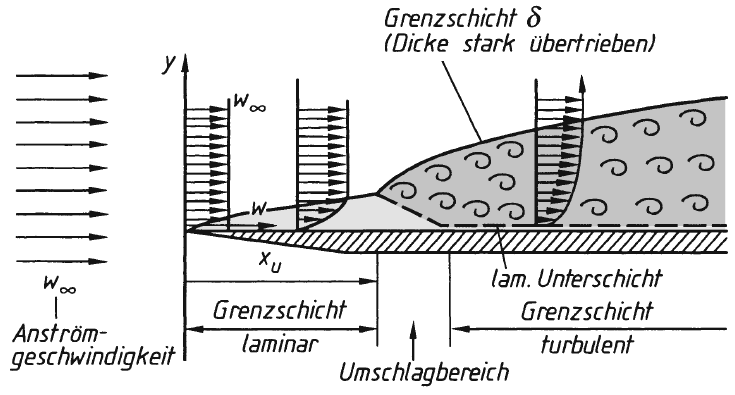
\includegraphics[width=0.7\textwidth]{Bilder/grenzschichttheorie}
	\caption{Veranschaulichung der Grenzschichttheorie \cite{Boeswirth2014}}
	\label{img:grenzschichttheorie}
\end{figure}

Und hier noch eine Referenz zur Einleitung, siehe Kapitel \ref{sec:einleitung}.\\
Danach noch eine Tabelle als Beispiel.\\

Im folgenden Abschnitt sollen die chemischen Reaktionen untersucht werden, die zu Ablagerungsprodukten führen. Die wichtigen festen Folgeprodukte der Harnstoffzersetzung sind in Tabelle \ref{tbl:harnstofffolgeprodukte} gelistet.

	\nomenclature[cBIU]{NH\textsubscript{2}-CO-NH-CO-NH\textsubscript{2}}{Biuret}
	\nomenclature[cTRIU]{NH\textsubscript{2}-CO-NH-CO-NH-CO-NH\textsubscript{2}}{Triuret}
	\nomenclature[cCYA]{C\textsubscript{3}N\textsubscript{3}(OH)\textsubscript{3}}{Cyanursäure}
	\nomenclature[cAMELID]{C\textsubscript{3}N\textsubscript{3}(OH)\textsubscript{2}NH\textsubscript{2}}{Ammelid}
	\nomenclature[cAMELIN]{C\textsubscript{3}N\textsubscript{3}OH(NH\textsubscript{2})\textsubscript{2}}{Ammelin}
	\nomenclature[cMEL]{C\textsubscript{3}N\textsubscript{3}(NH\textsubscript{2})\textsubscript{3}}{Melamin}

\begin{table}[h]
	\centering
	\begin{tabular}{C{2,2 cm}|C{5,4 cm}|C{2,8 cm}|C{2,8 cm}}
		\centering \textbf{Produkt} &
		\centering \textbf{chemische Formel} &
		\centering \textbf{Schmelzpunkt} &
		\centering \textbf{Zersetzungs-beginn}\tabularnewline
		\hline
		Biuret & NH\textsubscript{2}-CO-NH-CO-NH\textsubscript{2} & 193\,°C & 193\,°C\\
		Triuret & NH\textsubscript{2}-CO-NH-CO-NH-CO-NH\textsubscript{2} & 231\,°C & ca. 220\,°C\\
		Cyanursäure & C\textsubscript{3}N\textsubscript{3}(OH)\textsubscript{3} & 320\,°C - 330\,°C & ca. 220\,°C\\
		Ammelid & C\textsubscript{3}N\textsubscript{3}(OH)\textsubscript{2}NH\textsubscript{2} &  & 270\,°C\\
		Ammelin & C\textsubscript{3}N\textsubscript{3}OH(NH\textsubscript{2})\textsubscript{2} &  & 300\,°C\\
		Melamin & C\textsubscript{3}N\textsubscript{3}(NH\textsubscript{2})\textsubscript{3} & 354\,°C - 357\,°C & 354\,°C - 357\,°C\\
		
	\end{tabular}
	\caption{Wichtige Folgeprodukte der Harnstoffzersetzung, chemische Formeln und charakteristische Temperaturen, zusammengestellt aus \cite{Brack2016}.}
	\label{tbl:harnstofffolgeprodukte}
\end{table}
 

	\nomenclature[i0]{0}{normiert}
	\nomenclature[rW]{$w$}{Tangentialgeschwindigkeit $\left[\frac{m}{s}\right]$}
	\nomenclature[rR]{$R$,$r$}{Radius [m]}
	\nomenclature[cSTICKSTOFFMO]{NO}{Stickstoffmonoxid}	
	\nomenclature[cSTICKSTOFFDI]{NO\textsubscript{2}}{Stickstoffdioxid}
	\nomenclature[cAMMONIAK]{NH\textsubscript{3}}{Ammoniak}
	\nomenclature[cKOHLENMONO]{CO}{Kohlenstoffmonoxid}
	\nomenclature[cKOHLENDIO]{CO\textsubscript{2}}{Kohlenstoffdioxid}
	\nomenclature[rT]{$T$}{Temperatur [K]}
	\nomenclature[rC]{$c$}{Schallgeschwindigkeit $\left[\frac{m}{s}\right]$}
	\nomenclature[rM1]{$M$}{molare Masse $\left[\frac{g}{mol}\right]$}
	\nomenclature[rN]{$n$}{Stoffmenge [mol]}
	\nomenclature[rM3]{$\dot m$}{Massenstrom $\left[\frac{kg}{h}\right]$}
	\nomenclature[rNPUNKT]{$\dot n$}{molarer Strom $\left[\frac{mol}{h}\right]$}
	\nomenclature[rL]{$L$}{charakteristische Länge [m]}
	\nomenclature[gl]{$\alpha$}{Wärmeübergangskoeffizient $\left[\frac{W}{m²*K}\right]$}
	\nomenclature[iFl]{Fl}{Fluid}
	\nomenclature[iW]{W}{Wand}
	\nomenclature[iMSCR]{mSCR}{modulare SCR-Strecke}
	\nomenclature[rNu]{\textit{Nu}}{Nusselt-Zahl [-]}
	\nomenclature[rr]{$r$}{Ortskoordinate [m]}
	\nomenclature[gt]{$\vartheta$}{Temperatur [°C]}
	\nomenclature[gl]{$\lambda$}{Wärmeleitkoeffizient $\left[\frac{W}{m*K}\right]$}
	\nomenclature[rQPUNKTk]{$\dot q$}{spezifischer Wärmestrom $\left[\frac{W}{m²}\right]$}


\section{Zusammenfassung und Ausblick}
\label{sec:zusammen-ausbl}
Hier kommt die Zusammenfassung und der Ausblick.

\newpage
\pagenumbering{roman}
\setcounter{page}{1}
\addcontentsline{toc}{section}{Literaturverzeichnis}
\bibliography{LiteraturquellenStudienarbeit}

\newpage
\appendix
\section{Anhang: Ergänzende Dokumente zu Blabla}

\subsection*{Anhang Titel 1}
\label{sec:anhang-1}
%\begin{figure}[h]
%	\centering
%	\includegraphics[width=0.99\textwidth]{Bilder/Anhang/meinbild1}
%\end{figure}
Hier kommt Anhang 1
\pagebreak

\subsection*{Anhang Titel 2}
\label{sec:anhang-2}
%\begin{figure}[h]
%	\centering
%	\includegraphics[width=\textwidth]{Bilder/Anhang/meinbild2}
%\end{figure}
Hier kommt Anhang 2
\pagebreak


\end{document}